\documentclass[a4paper,11pt]{article}

\usepackage[top=2cm,bottom=2cm,left=2cm,right=2cm]{geometry}
\usepackage[pdftex]{graphicx} %per poter inserire le figure
\usepackage{amssymb,amsmath,amsthm,amsfonts}
\usepackage{xspace}
\usepackage{tabularx}
\usepackage{indentfirst}
\usepackage{subfigure}
\usepackage[small]{caption}
\usepackage{eucal}
\usepackage{eso-pic}
\usepackage{url}
\usepackage{booktabs}
\usepackage{afterpage}
\usepackage{parskip}
\usepackage{listings}
\usepackage{fancyhdr}
\usepackage{textcomp}
\usepackage{cite}
\usepackage{multirow}
\usepackage[utf8]{inputenc}   %per riuscire a scrivere gli accenti
%\usepackage[italian]{babel}   %per riuscire a scrivere gli accenti
\usepackage[english]{babel}
\usepackage{setspace}
\usepackage{tablefootnote}
\pagestyle{fancy} 
\usepackage{xcolor,colortbl}
\usepackage[compat=1.1.8]{tikz-feynman}
\usepackage{amsmath}
\usepackage{minted}

\title{Phase 2 GT Final-OR Documentation}
\author{Gabriele Bortolato}

\begin{document}

\maketitle

\section{Introduction}
\begin{figure}[h]
    \centering
    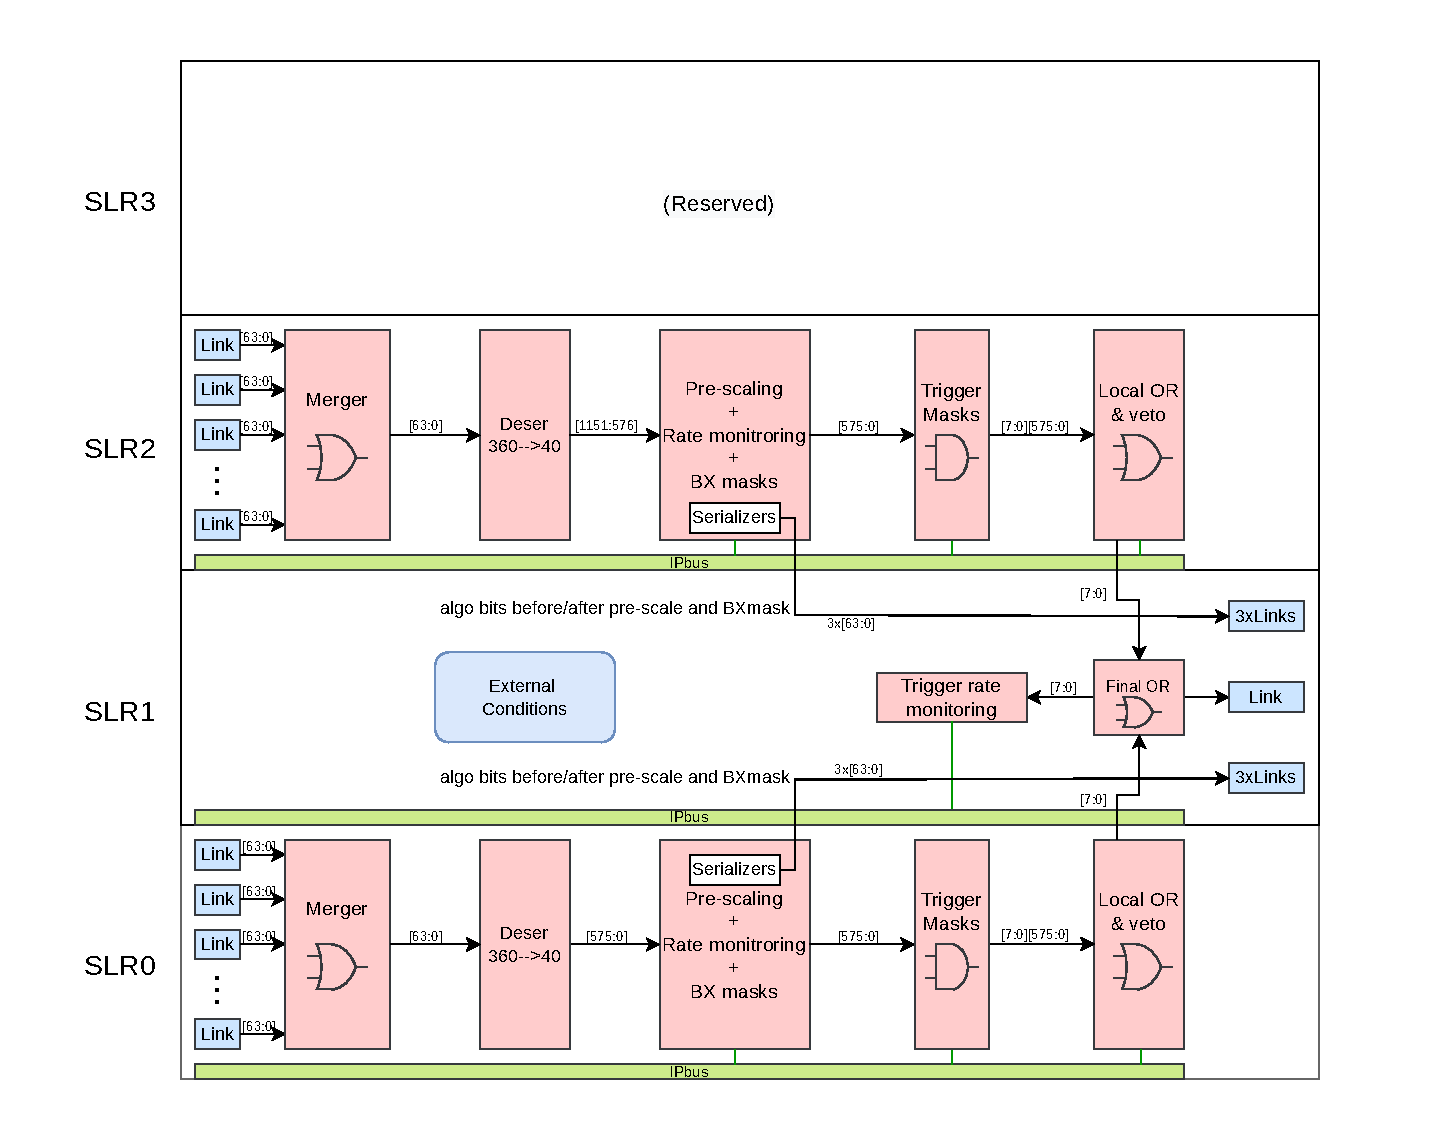
\includegraphics[width=0.95\textwidth]{Images/Finor_layout_SLR201.pdf}
    \caption{Caption}
    \label{fig:Finor_overview}
\end{figure}

\section{Modules}

In this section main modules will be described in detail, starting from what the data see first up to the last OR. Only the modules within the EMP payload will be described, if more information about EMP framework is need visit the EMP website (\textcolor{red}{putref}) or the GitLab repository (\textcolor{red}{putref}).   

\subsection{Link merger}

\begin{figure}[h]
    \centering
    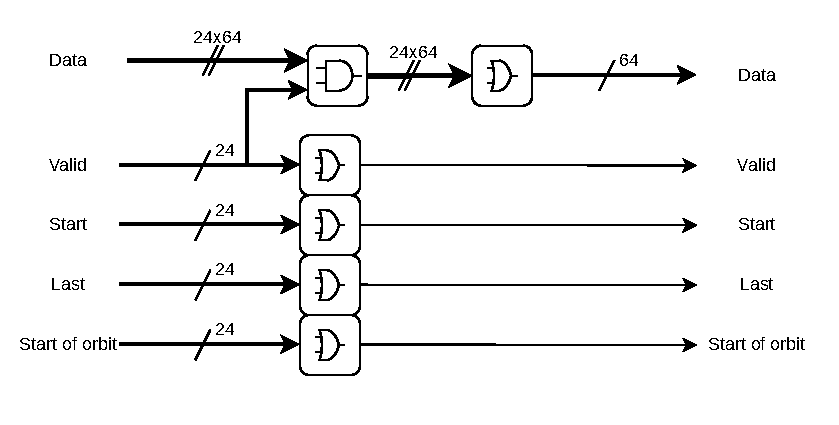
\includegraphics[width=0.85\textwidth]{Images/Modules/Link_merger.pdf}
    \caption{Caption}
    \label{fig:Merger}
\end{figure}

The link merger has to take as input the data links, coming from GT-Algorithm boards, and merge them into a single data link. To achieve this each metadata bits are OR-ed together, i.e. all the valid bits are "merged" into a single bit. The data straem is merged in a similar way OR-ing together the data bits, but they are set to zero according to its valid bit this is done per link basis.  

An issue that may arise is the fact that if one of the link is not aligned it will produce a wrong output. To tackle this issue a link mask is applied before the merging step, if a specific link is masked it will be set to a NULL value which means all metadata and data bits are set to 0.  
Such link mask value can be accessed via IPbus.

\subsection{Deserializer}

\begin{figure}[h]
    \centering
    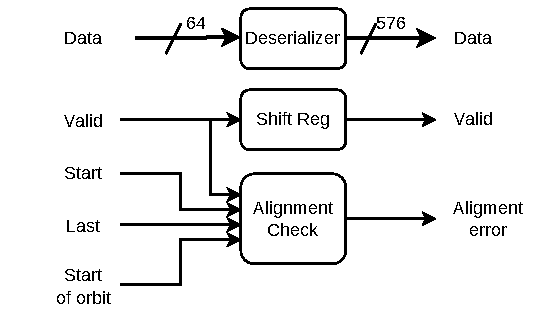
\includegraphics[width=0.75\textwidth]{Images/Modules/Deserializer.pdf}
    \caption{Caption}
    \label{fig:Deser}
\end{figure}

The deserializer module has to translate the 64-bit 360 MHz stream into 576-bit 40 MHz stream, to achieve this a frame counter starts count when link valid is asserted, it will count from 0 to 8 and start over.  

At different frame counter values the 64-bit word is placed in different position within the 576-bit vector.  
A shift register is used to delay the incoming valid bit by exactly nine 360MHz clock cycles.  

An alignment check is performed on the input metadata bits to verify if they behave as expected, e.g. start-of-orbit signals happens when the frame counter is 0.

\subsection{Pre-scaler}
The pre-scale module developed by the Global Trigger group for the $\mu$GT has been modified, but the main logic stayed the same \cite{uGT}. The new module has been heavily optimized to reduce the resource foot print in order to reach the goal of 1152 total algorithms. Such optimization range from simple logic rearrangement to signal vectorization. The loading of the pre-scaler values is pictured in Fig. \ref{fig:Pre-scaler-load} where it is used a dual port ram to store the values, at each luminosity section the RAM is read and the values are stored in a register array, in the next luminosity section if the request update flag is asserted the factors are loaded inside the algo-slices.

Every algorithm has a pre-scaler with a pre-scale factor 24 bits wide\footnote{This number can be increased up to 32 bits}. This module reduces the trigger-rate of the incoming algorithm by a given factor that can be set via software. For example a factor of 3 lets every third trigger pass blocking the first two.\newline 
A new feature introduced in 2019 is the possibility to set a fractional factor, each factor will be defined with an integer part and two digit fractional values. An example waveform with a factor of $1.75$ is shown in Fig. \ref{fig:prescaler}.\newline
The counter's increment of each algorithm assertion is $100$, in fact with two fractional digit this corresponds to exactly $1$. The factor of this example is $1.75$, if the counter plus the increment is greater or equal to the pre-scale factor the algo\_prescale flag is asserted and the counter is decreased by the pre-scale factor value.

\begin{figure}[h]
    \centering
    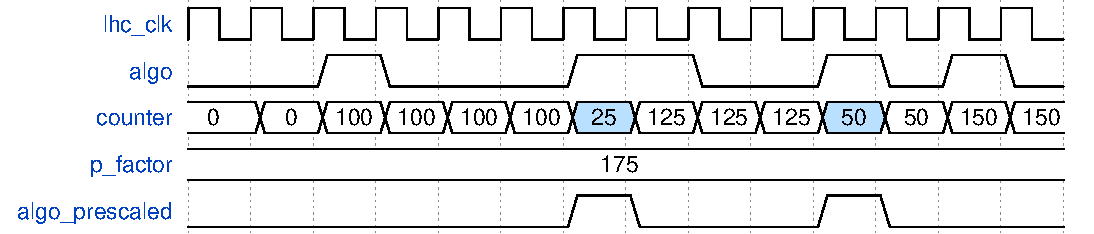
\includegraphics[width=0.93\textwidth]{Images/Modules/Prescaler_wf.pdf}
    \caption{Pre-scaler counter increment waveform.}
    \label{fig:prescaler}
\end{figure}

\subsection{Rate counter}

The rate counters are used to extract the rate of each algorithm for monitoring purposes, in fact as was described in section \ref{sec:L1T}, the level-1 trigger has a maximum accept rate and it is useful to have a monitor to spot potential rate mismatch with the expected values. 

The counter is increased at each LHC clock cycle if the input algorithm is asserted while the reset condition is the start of a luminosity section or an external signal. Right before the reset its value is stored in a register and monitored by the experiment control room. In the implementation used in this work these rate counters are 32-bits wide.

Four rate counter are instantiated for each algorithm, one before the pre-scale, one after the pre-scale, one after the preview pre-scale and one post dead-time. The post dead-time counter is a slight variation of the other three, it increments the register only if the algorithm and the delayed L1A signal are both asserted,  which means that only the algorithm assertions that can save the event are taking into account.


\subsection{BX mask}
The BX mask, as the name suggests, will exclude a given algorithm in a given BX number. The implementation is rather simple, in fact it is implemented as a dual port RAM, one port is connected to the programmable logic the other on is accessible via IPbus. This RAM has to be 3564 deep and 1152 wide, the first limitation is related to the number of BX in one orbit, the second limitation is related to the number of running algorithms. The IPbus suite can manage memory resource A32/D32 which means that 1152/32=36 dualport ram in parallel\footnote{18 per monitoring SLR}.  

The BX number is used as address and the content of this wide RAM is the mask of that specific BX number.

\subsection{Algo slice}

\subsection{Local-OR and Trigger type masks}
Unlike $\mu$GT the Phase-2 GT will have multiple trigger bits which are selected to tackle different Physics, an example of 8 trigger bits is given in the table \ref{tab:trigger_types}.  


\begin{table}[ht] \
  \begin{minipage}[b]{0.5\linewidth}
    \centering
    \begin{tabular}{|c|c|}
    \hline
    Index & Trigger type      \\
    \hline
    0 & Stadard Physics     \\
    1 & Zero Bias           \\
    2 & Minimum Bias            \\
    3 & High Priority       \\
    4 & Long-lived particle (LLP)    \\
    5 & First event of a 2-event LLP   \\
    6 & Second event of a 2-event LLP  \\
    7 & Periodic validation event      \\
    \hline
    \end{tabular}
    \caption{Example of 8 different trigger bits}
    \label{tab:trigger_types}
    \vspace{4ex}
  \end{minipage}%%
  \begin{minipage}[b]{0.5\linewidth}
    \centering
    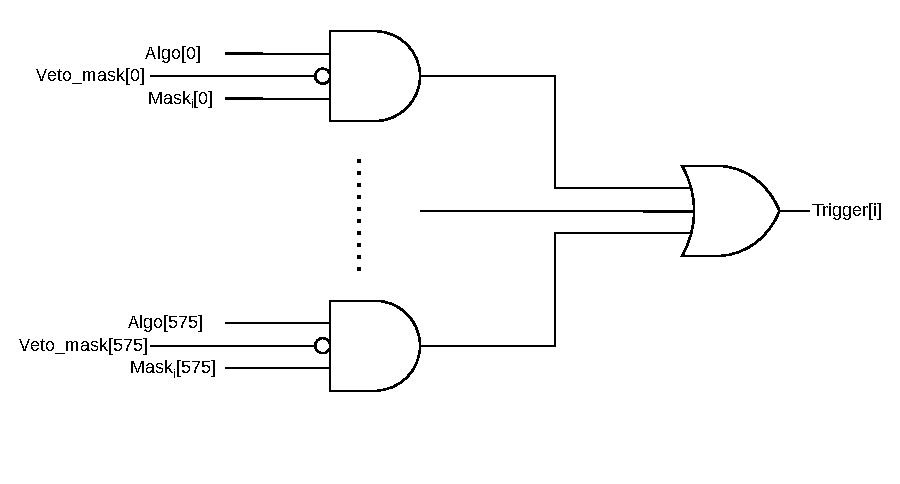
\includegraphics[width=0.95\textwidth]{Images/Modules/Trigger_mask.pdf}
    \captionof{figure}{Schematic view of the extraction of the i-esim local trigger bit.}
    \label{fig:TriggMasks}
    \vspace{4ex}
  \end{minipage} 
\end{table}

To extract such trigger bits, first a mask is applied to the whole algorithm vector selecting only a fraction of the 576 bits\footnote{This process is done in each monitoring SLR} if an algorithm act as veto it will be excluded from the final OR computation, then local OR\footnote{Local in the sens that is computed in each SLR} is computed to each masks results, such outputs are the local trigger bits. The masks are loaded via an IPbus dual port RAM with the exact same structure of the pre-scale factors. A diagram of such process is shown in Fig. \ref{fig:TriggMasks}

\subsection{Veto}

Veto mask is simliar to the trigger masks the only difference is teh fact that it is need only one mask, the latter is loaded via IPbus to identify which algorithms will act as veto. If any of these algorithms is asserted the trigger with veto will be bound to zero, in hardware this is done with an AND gate.

\begin{figure}[h]
    \centering
    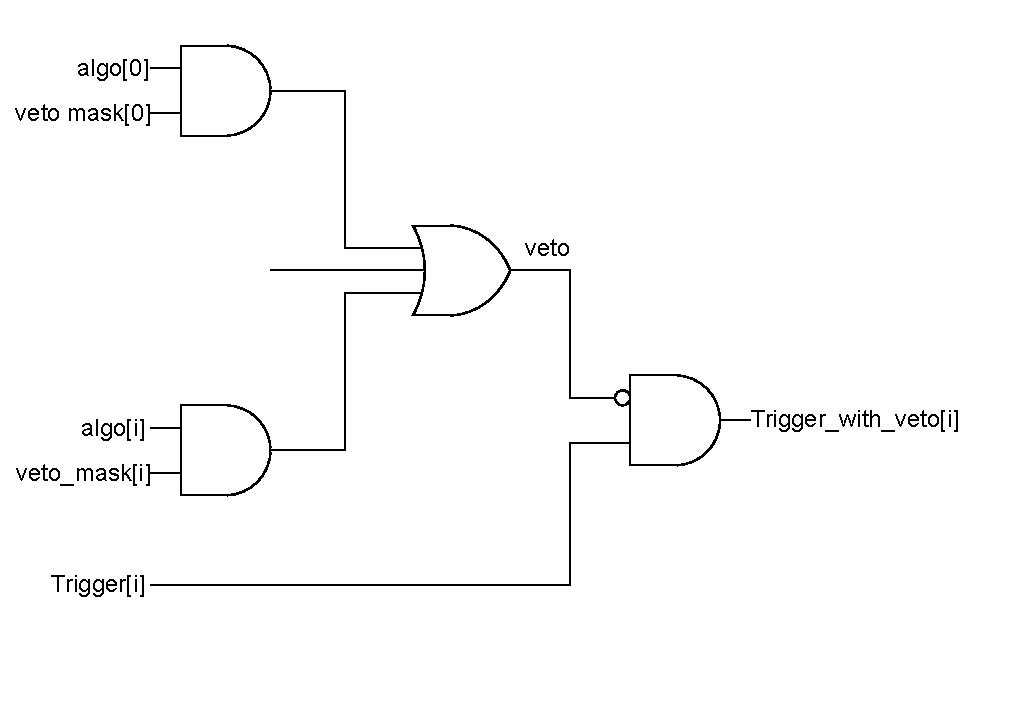
\includegraphics[width=0.8\textwidth]{Images/Modules/Veto.pdf}
    \caption{Veto logic.}
    \label{fig:VetoMask}
\end{figure}

\subsection{Final-OR}

The final OR is done combining the signals from the two monitoring SLRs. Each SLR outputs the local or (8-bits wide), the local or preview (8-bits wide) and the local veto.

\begin{figure}[h]
    \centering
    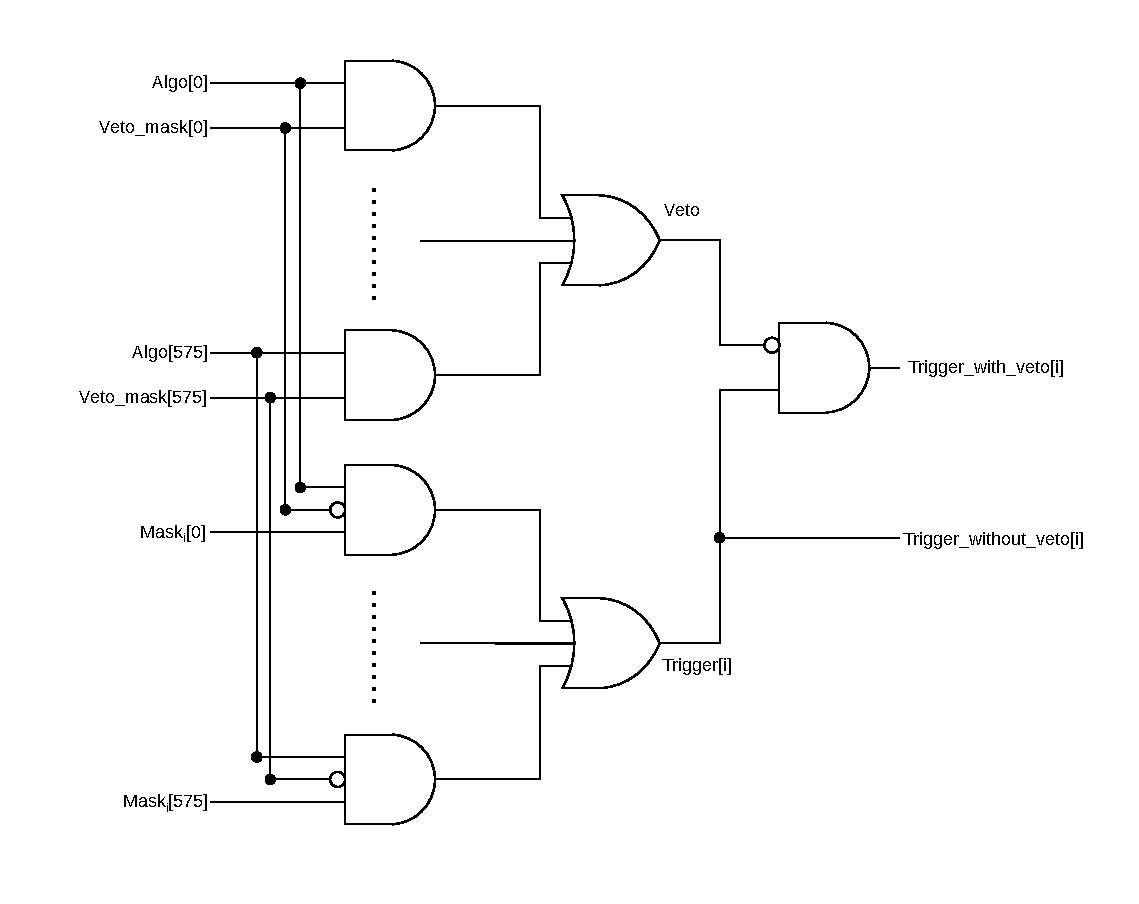
\includegraphics[width=0.8\textwidth]{Images/Modules/Trigger_Veto.pdf}
    \caption{Trigger and veto mask logic.}
    \label{fig:VetoMask}
\end{figure}

\subsection{Output interface}
\textcolor{red}{To be discussed}


\section{Payload IPbus tree}

\section{Pre-scale column loading}
Due to the high number of monitored algorithms, the pre-scale columns cannot be loaded form SW with generic IPbus register banks. In fact, multiple issues arise doing so, the obvious solution is to use dual port RAMs (DPRAM). The drawback of such approach is the time required to read the content of the DPRAM, in this case the column is split in two monitoring SLRs with 576 factors which means $\sim$14.4$\mu s$ read time required.  

In FW it are present two banks of registers, one to store the values from the RAM and one that is updated only at the begining of a luminosity sections, a scheme of such tructure is given in Fig. \textcolor{red}{ref}

\begin{figure}[h]
    \centering
    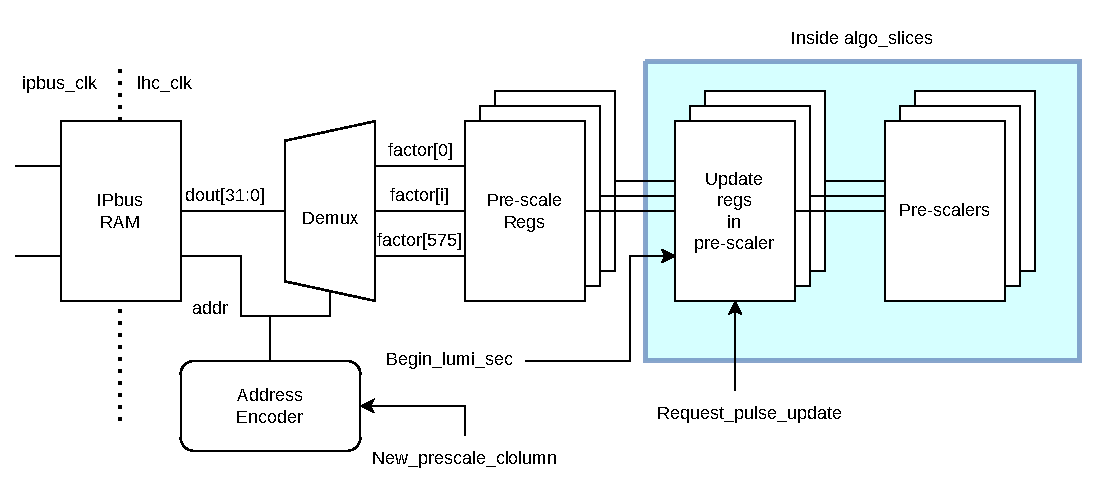
\includegraphics[width=0.8\textwidth]{Images/Prescale-section/Prescaler_load.pdf}
    \caption{Caption}
    \label{fig:my_label}
\end{figure}

Pre-scale column can be update only at the begin of a luminosity section, in this way a column is retained throughout the whole luminosity section. 
The pre-scale column loading follow these steps:
\begin{itemize}
    \item A new column is loaded into the IPbus RAM via SW
    \item A load flag is pulsed via SW
    \item If a load flag is sensed in the HW a FSM \textcolor{red}{put ref} it will trigger the start of the loading routine
\end{itemize}
The loading routine is depicted in the Fig. \textcolor{red}{put ref}.
\begin{table}[]
    \centering
    \begin{tabular}{c|c|c}
        State & Change conditions & Output \\
        \hline
        \multirow{2}{*}{Idle}  & \multirow{2}{*}{Load flag = '1'} & Request\_update='0' \\
        && addr = 0 \\
        \multirow{2}{*}{Check} & orbit\_nr[LS\_BIT-1:0] $\leq$ & Request\_update='0' \\
        & $2^{LSBIT}-2$ & addr = 0 \\
        \multirow{2}{*}{Load} & \multirow{2}{*}{addr $\geq$ RAM\_DEPTH-1} & Request\_update='0' \\
        && addr = addr+1 \\
        \multirow{3}{*}{Done} & \multirow{3}{*}{Only one clock cycle} & Request\_update='1' \\
        && addr = 0 \\
        && LS\_mark = LS\_nr+1 \\
    \end{tabular}
    \caption{Caption}
    \label{tab:my_label}
\end{table}
The Check state evaluates if the column can be loaded safely in the register bank, avoiding any possible partial loading, in fact if a read routine starts right before the begin of a luminosity section the factors towards the end are not updated. The check is done on the orbit number , if this number is not the last orbit or the one before it the reading procedure can take place otherwise it will wait the next luminosity section. 

\subsection{SW code example}
Random pre-scale factors set in SW example:

\begin{minted}{python}
# Pre-scale default factors
prsc_fct      = np.uint32(100 * np.ones((2,576)))  # 1.00
prsc_fct_prvw = np.uint32(100 * np.ones((2,576)))  # 1.00
# Spit indexes in two SLR subsets
index_low  = index[np.where(index < 576)[0]]
index_high = index[np.where(index >= 576)[0]]
#random assign 
prsc_fct[1][np.int16(index_high - 576)] = 
    np.uint32(np.random.randint(100, 2 ** 24, len(index_high)))
prsc_fct[0][np.int16(index_low)] = 
    np.uint32(np.random.randint(100, 2 ** 24, len(index_low)))
#load the data into the IPbus RAM
HWtest.load_prsc_in_RAM(prsc_fct, PRESCALE_INDEX)
#same routine for the preview
prsc_fct_prvw[1][np.int16(index_high - 576)] = 
    np.uint32(np.random.randint(100, 2 ** 24, len(index_high)))
prsc_fct_prvw[0][np.int16(index_low)] = 
    np.uint32(np.random.randint(100, 2 ** 24, len(index_low)))
HWtest.load_prsc_in_RAM(prsc_fct, PRESCALE_PREVIEW_INDEX)
\end{minted}

New column flag SW example:

\begin{minted}{python}
#Send the new column flag 
HWtest.send_new_prescale_column_flag()
time.sleep(2)
#Read the Lumi section mark
ls_prescale_mark = HWtest.read_lumi_sec_prescale_mark()
print("SLR 2 pre-scale column loaded mark = %d" % ls_prescale_mark[0])
print("SLR 3 pre-scale column loaded mark = %d" % ls_prescale_mark[1])
\end{minted}
    
\section{Trigger types masks and veto loading}

The trigger type masks and the veto mask work in a similar fashion, but the RAM depth changes in relation to the bits that needs to be sent, a summary of registers required per SLR is given in the table \textcolor{red}{put ref}.
\begin{table}[]
    \centering
    \begin{tabular}{c|c|c|c|c}
    Reg name & 32-bit Regs & RAM Depth & RAM Width \\
    \hline
    Pre-scale &  576 & 1024 & 32  \\ 
    Pre-scale preview &  576 & 1024 & 32 \\ 
    Trigger type masks &  $\frac{576}{32}\times 8 = 144 $ & 256 & 32 \\ 
    Veto mask &  $\frac{576}{32}\times 1 = 18 $ & 32 & 32\\ 
    BX masks &  $\frac{576}{32}\times 3564 = 65772 $ & 4096 & 576 \\
    Algo rate counters ($\times 4)$ &  576 & 1024 & 32 \\ 
    Trigger rate counters ($\times 8)$ &  8 & 8 & 32 \\ 
    
    \end{tabular}
    \caption{Caption}
    \label{tab:my_label}
\end{table}




\section{Rate counters values dumping}
\begin{figure}
    \centering
    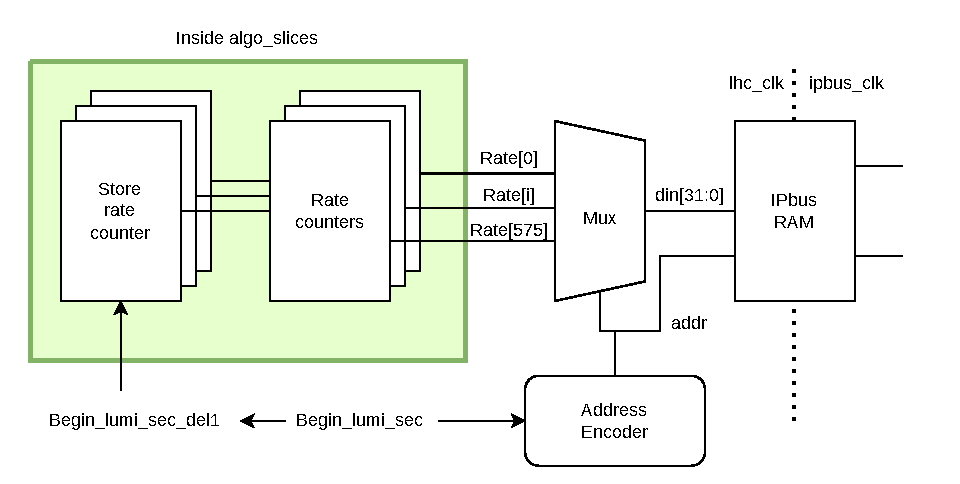
\includegraphics[width=0.8\textwidth]{Images/Prescale-section/Rate_cnt_read.pdf}
    \caption{Caption}
    \label{fig:my_label}
\end{figure}


\section{Final Or standalone test}
A set of tests have been developed to check the Final-OR design correct behaviour. Such tests are unitary test in the sense that on a specific feature is tested each time. The tests developed are the following:
\begin{itemize}
    \item \textbf{Pre-scaler test}: It will check if the pre-scalers and pre-scalers preview works as expected
    \item \textbf{Trigger type masks test}: Here the trigger type masks logic is evaluated.
    \item \textbf{Veto mask test}: Similar to the Trigger type mask, but in this case only the veto mask is tested.
    \item \textbf{BX mask test}: test to evaluate the correct behaviour of the BX mask.
\end{itemize}
In the following sections each test is explained in detail.

\subsection{Pre-scaler test}
The EMP framework allows the injection of patternfiles directly on the datapath buffers, such buffers are limited in depth, in fact it is possible to inject up to 1024 frames, or 113\footnote{$int(\frac{1024}{9})=113$, the link clock is 360MHz, in a BX 9 clock cycles are present} packets with TMUX=1.  

As was mentioned in section \textcolor{red}{put ref} the Final-OR can manage up to 1152 algorithms. To produce a patterfiles it is necessary to first decide where (in terms of BXs) and which algorithm will fire, to do so a matrix 1152x113 is produced. The entries of such matrix can be either [\textit{True,1}] or [\textit{False,0}], the user can select the probability that an algorithm fires in a specific BX, this probability is constant throughout the whole matrix.

\[
Matrix_{algo}=
\underbrace{\begin{bmatrix}
    0  & \cdots & 1 & \cdots & 1      \\
    \vdots  & \ddots & \cdots & 0 & \vdots       \\
    0  &\cdots & 0 & \cdots & 1       \\
    \vdots  &1&\cdots & \ddots & \vdots       \\
    0  & \cdots & 0 & \cdots & 1       
\end{bmatrix}}_{113}
\begin{tabular}{l}
$\left.\lefteqn{\phantom{\begin{matrix} 0\\ \ddots\\ 0\\ \ddots\\ 0\  \end{matrix}}}\right\}1152$
\end{tabular}
\]

Once the matrix is produced a pattern files is generated starting from the position of such algorithm indexes and available links. The pattern file is produced distributing the signals within the links pool.  

The EMP framework will repeat the pattern file once every orbit, wich means that during a \textbf{luminosity section} the pattern is played $2^{LSBIT}$ times. The next step the expected unprscaled counts are extracted for each algorithm, to do so the columns are summed together resulting in a 113-wide vector.

\[
\begin{bmatrix}
    0  & \cdots & 1 & \cdots & 1      \\
    \vdots  & \ddots & \cdots & 0 & \vdots       \\
    0  &\cdots & 0 & \cdots & 1       \\
    \vdots  &1&\cdots & \ddots & \vdots       \\
    0  & \cdots & 0 & \cdots & 1       
\end{bmatrix}
\rightarrow \vec{R} = 
\begin{bmatrix}
    10      \\
    \vdots      \\
    32     \\
    \vdots      \\
    22       
\end{bmatrix}  
\begin{tabular}{l}
$\left.\lefteqn{\phantom{\begin{matrix} 0\\ \ddots\\ 0\\ \ddots\\ 0\  \end{matrix}}}\right\}1152$
\end{tabular}
\]
The counts before pre-scale are computed with the formula:
\begin{equation}
    Counts = \vec{R} \cdot  2^{LSBIT}
\end{equation}

Then a pre-scale column is loaded into the firmware, such column can be either randomly generated or with equally sapaced values starting from $1.00$ to $\frac{2^{24}-100}{100}=167771.16$. The theoretical counts after the pre-scalers are evaluated with the formula:
\begin{equation}
    Counts = (\vec{R} \cdot  2^{LSBIT}) \oslash \vec{C} 
\end{equation}

Finally the firmware is loaded into the board and the rate counters are read and compared against the theoretical ones, if the mismatch is greater that 1 an error is raised and the test is failed.

\subsection{Trigger type test}

The trigger type masks test works in a similar way, but the final or counts are checked. To do so the algo matrix is split it 8 sub matrices  maintaining the 113 witdh, which mean that 8 subsets of algorithms are selected from the pool.  

From these selections 8 different trigger type mask are extracted and saved to file to be passed to the RateChecker script.

Finally the column-wise OR is computed to such matrices resuling in a 8 113-wide vectors, the last step is to compute the element sum of suc vectors resulting in 8 different counts for each trigger type. Then the results are compared against the hardware extract ones.

\textcolor{red}{put image}


\subsection{Veto mask test}

Starting from a generated algo matrix a number of veto algorithms are extracted and a veto mask is produced, then the Final-OR counts are computed with and without the veto. In this test all trigger type mask are set as pass through\footnote{As it was mentioned these are unitary tests, so they will test only one feature}.


\subsection{BX mask test}

The test starts again with a algorithm matrix, then a BX mask matrix is produced in a similar way, in this case the probability of assertion is much grater (40\%). Then the two matrices are bit-wise AND together to get the algorithm BXmasked matrix. From the algorithm matrix is extracted the input patternfile to sent to the board, from the BXmask matrix is extracted the relative BX masks and from the algorithm BXmasked matrix counts before pre-scalers are evaluated. Such counts are then check against the HW results. 

\subsection{Suppress trigger during calibration test}

\textcolor{red}{Not yet defined}

\end{document}
